\documentclass[11pt,letterpaper]{article}
\usepackage[margin=1in]{geometry}
\usepackage{amsmath}
\usepackage{graphicx}
\usepackage{algpseudocode}
\usepackage{framed}
\usepackage{hyperref}

\title{Automated Intersection Modeling}
\author{Albert Ou, Praagya Singh, Ross Yeager}
\date{May 17, 2013}

\begin{document}

\maketitle

\section{Introduction}
Once limited to the realm of science fiction, autonomous consumer vehicles, or driverless cars, present a very exciting opportunity for the application of interdisciplinary research from artificial intelligence, robotics, control theory, and embedded systems. Since the late 2000s, numerous advances have been made in the field. Prototypes have been researched and/or tested by Toyota, Nissan, and Audi. Three U.S. states have passed laws permitting autonomous vehicles. A world full of driverless cars presents a host of benefits, but much work is yet to be done before this becomes a reality.\\
The full assimilation of autonomous vehicles in daily life involves solving many subproblems such as ensuring safety, implementing error-free and robust control mechanisms, and building corresponding infrastructure. This includes the design of intersections that support and optimize for autonomous vehicles.  Traditional, four way intersections will need to be revamped: red-yellow-green switching will be rendered mostly obsolete, and traffic will be continuously directed at a much finer scale by an autonomous controller agent.

In this paper, we propose a model for such an intelligent, automated intersection of two lanes on each side, to facilitate efficient routing of a sampling of vehicles that are mostly autonomous. Our model, unlike some existing research, advocates for a centralized controller instead of a P2P protocol. This centralized controller will ensure safety (i.e. no collisions) and fairness. We will formalize the communications between the car and the central controller, provide the mathematical groundwork for the geometry of our intersection and the paths of the vehicles and analyze our results. We also provide a demonstrative model of our system using Ptolemy II. With our basic model we hope to provide groundwork for the development of a more robust solution. 


\section{Previous Work}

The Autonomous Intersection Management project at UT Austin investigated
control policies that divided the intersection into a grid of reservation
tiles.\cite{Dresner}

\section{Algorithms and Models}

\subsection{Vehicles}

In our autonomous intersection model, there were originally two types of vehicles that were defined: autonomous vehicles and human driven vehicles.  However, given the scope of the project, the vehicle types were reduced to autonomous vehicles only. The autonomous vehicles all take on the same physical characteristics in our model. These properties are explained in the following section.

\subsubsection{Vehicle Model Properties}

Typically, cars are classified into many different phycial categories.  For simplicity, our model utilizes the most common type of vehicle, the passenger car (denoted as type P vehicle).  We define vehicle characteristics based on the intersection properties, normally defined in local roadway laws and regulations.  In this project, minimum characteristics of type P cars require a minimum inside radius of 16 ft. from the inner edge of the lane \cite{Bureau}.  This is implemented in our model in the pathway equations.  In our model, vehicles have certain properties that are similar to those seen in the physical world.  Exceptions have been made to make the simulation tractible and because these exceptions are reasonable within the given model.  First, we model vehicles with the ability to instantaneously change velocity and place a requirement that they have a constant velocity within intersection.  All intersection route paths are 68 ft or less and allow for limited change in velocity in the physical world.  Because of this, a constant velocity model is reasonable.

Another property is that range of the constant velocity of each car must be between 20-40 MPH: $V \rightarrow V \in [20,40]$ \cite{Motorists}.  In the model, the velocity is randomly generated within this range, simulating cars entering the model at different speeds.  These speeds are seen in intersection documentation and are directly implemented into the vehicle properties. Vehicle entry times and route are also randomly generated in order to simulate the authentic intersection.  We require routes to be constant throughout intersection traversal; this follows from standard intersection traffic laws.  The route is randomly generated from two parameters: path and direction.  The direction parameter determines which direction (North, South, East, or West) that the car will enter from, and the path parameter defines which path the vehicle will take (left turn, straight from left lane, straight from right lane, or right turn) from the given direction.  These randomly generated parameters describe the car speed, entry time, and route in our model.

To implement our model, we used Ptolemy II.  Ptolemy limitations prevent dynamic instantiation of new actors during simulation.  This presented a challenge as an intersection model needs continuous vehicle flow.  In order to overcome this, we use the Multi-Instance Composite Actor to emulate dynamic instantiation.  The Multi-Instance Composite Actor allows for $N$ instances of the vehicle modal model within this actor.  Each modal model represents a vehicle that may be in the intersection.  The number of vehicles in the intersection at any given time is limited to, at most, $N$ vehicles.  Vehicles exit the system when their travelled distance is greater than the distance of the given route that they are assigned.  The simulation then regenerates new parameters for the car and a new entry time in which the car can re-enter the intersection, thus effectively creating continuous vehicle flow. The following figure shows a high level view of the overal system.

\begin{center}
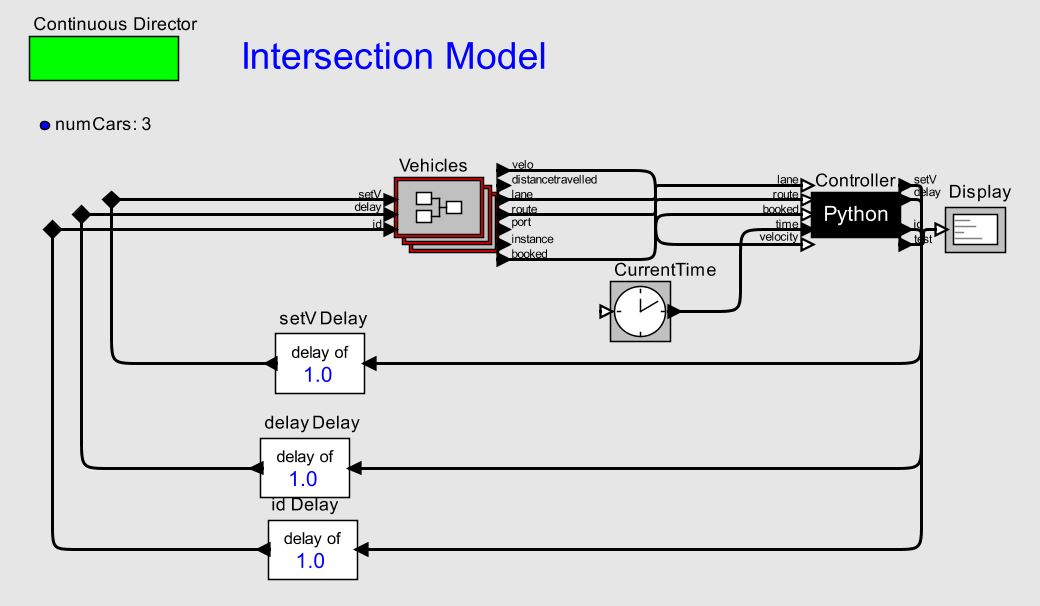
\includegraphics[width=0.65\linewidth]{diagram/ptolemy_system.jpg}
\end{center}

Within each instance of the Multi-Instance Composite Actor, there exist the random parameter generators as well as the modal model that houses the FSM Actor.  This can be seen below:
\begin{center}
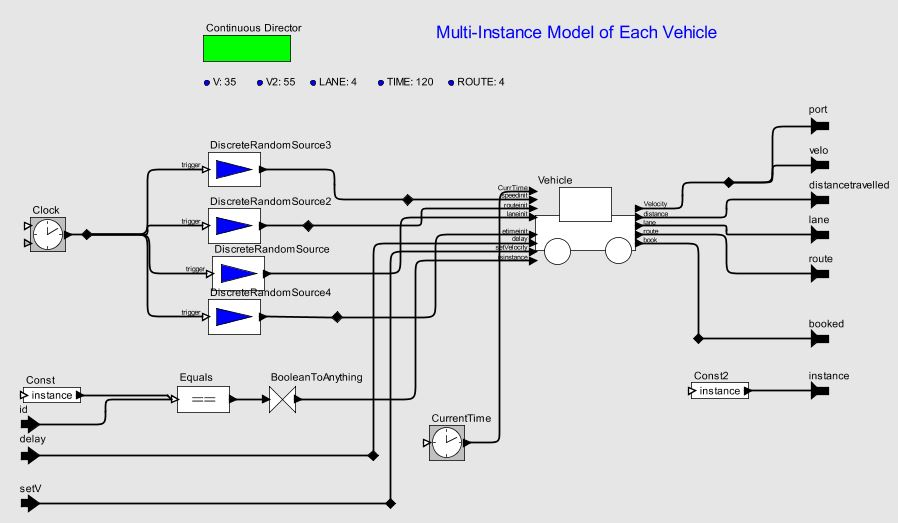
\includegraphics[width=0.65\linewidth]{diagram/ptolemy_multiinstance_actor.jpg}
\end{center}

Finally, there is the Modal Model.  This is a FSM Actor that contains the following states: \texttt{RUN, IDLE, ENTER, BOOK, GO,} and \texttt{WAIT}.  The \texttt{RUN} and \texttt{IDLE} states initialize the parameters of the vehicle and effectively instantiate a vehicle.  The car receives an initial route and velocity and waits in the \texttt{IDLE} state until its entry time has occurred.  Once the entry time has passed, the vehicle is in the \texttt{ENTER} state.  This state represents a vehicle entering the straightaway path before the intersection itself.  Given the vehicle's speed, the model calculates the time at which the vehicle will enter the intersection and sends this to the controller along with its route, speed, and instance.  The controller can then book the vehicle instance in this state, assigning it a different speed, a delay time at the intersection, or no command at all.  If a vehicle reaches the intersection (i.e. global time is greater than the time calculated in the straightaway), then we require that the vehicle stop at the intersection until it is booked.  Once a vehicle is booked (regardless of whether or not it has arrived at the intersection), it enters the \texttt{BOOK} state.  Here it waits until global time exceeds the straightaway time and then proceeds to the \texttt{GO} state.  This state models the vehicle going through the intersection itself, and outputs the distance travelled as well as the current velocity.  Once the vehicle has travelled the specified distance determined by its route, it goes to the \texttt{WAIT} state where the vehicle is set up for initialization again.  This loop continues as long as the simulation is running.  The FSM states can be seen in the following image:
\begin{center}
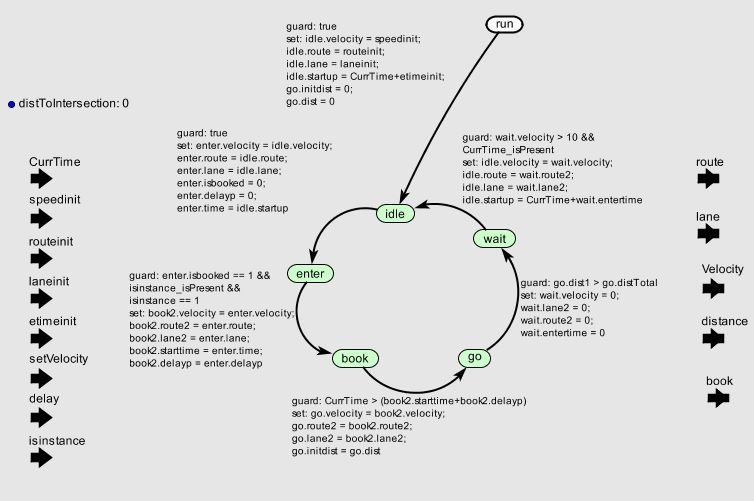
\includegraphics[width=0.65\linewidth]{diagram/ptolemy_vehicle_fsm.jpg}
\end{center}


\subsection{Conflict Detection}

To be effective at preventing traffic accidents, the controller for an
automated intersection must have an accurate method for detecting
collisions between individual vehicles before they arrive within minimum
stopping distance of the intersection.  Since the control problem
imposes hard real-time requirements, the primary concern was performance
that scaled gracefully with the number of participating vehicles.

As always, a balance must be found between fidelity and tractability.
For the highest accuracy, trajectories can be represented as
three-dimensional curves, with coordinates consisting of a temporal
component as well as spatial position.  Preventing collisions is
therefore equivalent to enforcing a lower bound on the Euclidean
distance between two such curves.  However, this method demands an
unrealistic amount of information about vehicular physics than is
obtainable during runtime.  We desire an alternative method that is
less numerically intensive, so it can be repeatedly applied as traffic
conditions evolve, but whose approximations do not compromise safety.

Focusing on the locations at which collisions are most likely to occur,
we begin with the concept of a \emph{traffic conflict point}, defined
as the point at at which multiple traffic flows may cross or merge.
As per normal regulations, we require that all vehicles adhere to
designated lanes when traversing the intersection, so that trajectories
can be bounded exactly.  Thus, the set of conflict points are determined
by the intersections between curves representing all legal paths of
vehicles.

We assume the following in our reference intersection model:
\begin{enumerate}
\setlength{\itemsep}{0pt}
\setlength{\parskip}{0pt}
\item Four-way symmetric intersection with orthogonal arms and
	perfect alignment
\item Open space without obstructions (e.g., pedestrians)
\item The total number of lanes at any exit approach equals the
	total number of lanes at any entrance approach.
\item Traffic lanes at an exit approach can only serve as the
	exit of lanes with the same lane number relative to
	the center line.
\end{enumerate}

Straight paths are simply modeled as vertical and horizontal lines.
The left-turn paths are circular arcs that circumscribe three control
points at the entrance, midpoint, and exit of the turn; the midpoints
are chosen to avoid conflicts with oncoming left-turn traffic.
For simplicity, U-turns are disallowed.  The right-turn paths are
circular arcs which subtend a right angle.\footnote{The actual path
equations are viewable on the presentation slides submitted along with
this report.}

In reality, vehicles are not point masses -- they occupy area.
We desire to enforce a minimum separation between vehicles traveling
on conflicting paths.  A \emph{traffic conflict zone} is defined as the
segment of a given path within a certain distance of a conflict point.
The initial and terminal points of a conflict zone are expressed as an
ordered pair of offsets/displacements along the curve, relative to the
start of the path.

The collision detection algorithm is therefore:
\begin{enumerate}
\setlength{\itemsep}{0pt}
\setlength{\parskip}{0pt}
\item Determine the set of conflict zones along the path.
\item Numerically integrate to determine when endpoints of conflict
	zones are crossed, yielding a set of time intervals.
\item For each conflict zone, check whether the corresponding time
	interval overlaps with that of any other active vehicle.
\end{enumerate}

It is important to note that conflict zones are static and therefore
need only to be calculated once during initialization.  Runtime does
not require knowledge about curvature of paths; only linear
displacements matter.  Reservations for a vehicle are thus scheduled
as time intervals during which it has exclusive access to the conflict
zones along its path.

\subsection{Controller}

The controller is a Python script that takes as input the car's current
lane, intended lane, velocity, and booking status, and outputs an
instruction in the form of a new velocity and delay. This instruction
implies that the car will stop at the intersection for $delay$ seconds, and
then proceed to continue along its intended path at a constant speed given
by new velocity. The controller guarantees that the car's trajectory,
assuming the instruction is properly followed, will be collision-free. The
controller receives requests and sends commands almost instantaneously to
system vehicles. For convenience in calculations, the controller also takes
as input the current time.

For a somewhat more realistic simulation, we decided to add a delayed
feedback to the controller output. Not only does this prevent a causality
loop and Zeno system, but it also models a real-life communication delay
between the controller and the vehicles. The controller also has a $id$
output, which enables multiplexer-like functionality such that the
controller is able to communicate with a particular vehicle in the
MultiInstanceCompositeActor.

The scheduling algorithm employed by the controller is as follows:

\begin{framed}
\centering\small
\begin{algorithmic}
\State {Initialize list of conflict zones and displacements along paths}
\For{each timestep $t$}
	\State $current \gets \text{all tokens received from Vehicle modal model}$
	\For{each $car$ in $current$}
		\If{$car$ needs reservation}
			\State {$v_\text{max} \gets$ maximum velocity
				$\in [ v_\text{current} \pm 10 ]$ that ensures safety}
			\If{$v_\text{max}$ exists}
				\State $v_\text{new} \gets v_\text{max}$
				\State $t_\text{delay} \gets 0$
			\Else
				\State $v_\text{new} \gets v_\text{current} + 10$
				\State $t_\text{delay} \gets$ end of latest reservation for all conflict zones
			\EndIf
			\State broadcast($v_\text{new}$, $t_\text{delay}$,
					$\text{id} \gets car\text{.id}$)
		\EndIf
	\EndFor
\EndFor
\end{algorithmic}
\end{framed}


\section{Technical Challenges}

\begin{itemize}
\setlength{\itemsep}{0pt}
\setlength{\parskip}{0pt}
\item Continuous car flow given static number of vehicles
\item Delivering controller commands to specified car instance
\item Continuous time solver time step evaluation issues
\item Hybrid system causality issues
\item Scalability
\end{itemize}

\section{Results}

\begin{itemize}
\setlength{\itemsep}{0pt}
\setlength{\parskip}{0pt}
\item Functional hybrid model
\item Continuous vehicle flow with static vehicle set
\item Centralized responsive controller
\item Rigorous intersection path definitions
\item Multiplexed communication to vehicles
\end{itemize}

\section{Future Work}

\begin{itemize}
\setlength{\itemsep}{0pt}
\setlength{\parskip}{0pt}
\item Investigate resource scheduling algorithms for optimization
\item Introduce non-zero vehicle acceleration into the model
\item Add support for vehicles with human drivers
\end{itemize}

\section{Team Roles}
\subsection{Albert Ou}

Albert was responsible for developing the collision detection algorithm.
In particular, he contributed the idea of conflict zones, defined the
intersection geometry, and formalized the path equations.
He also typeset the majority of the presentation slides.

\subsection{Praagya Singh}

\subsection{Ross Yeager}
Ross, along with all members, helped define the overall system problem and assumpions, and he was specifically in charge of designing and modelling the entire vehicle model.  
He created the Ptolemy system consisting of Multi-Instance Composite actors that allowed for a scalabile system with respect to the number of cars in the intersection.  
He created a the system that allowed for continous vehicle flow as well as the FSM that defined vehicle behavior.



\section{Conclusion}
%\subsection{Course Application}
In order to analyze and simulate our model, Ptolemy modelling software was used.  This tool allows for the creation of hybrid systems such as those seen in the autonomous roadway.  We used Modal Models for the vehicles represented in the system, and had to implement non-zero delay feedback loops in order to prevent a zeno system (both subject examined in class).  Furthermore, we simulated the basics of any standard system: a controller and environment of which it controls.
%\subsection{Feedback}

Useful topics covered in class and used in this project include:
\begin{itemize}
\setlength{\itemsep}{0pt}
\setlength{\parskip}{0pt}
\item Hybrid Systems
\item Finite Automata
\item Zeno Systems
\item Modeling Tools; Ptolemy II
\item Continuous ODE Solvers
\end{itemize}



\newpage
\begin{thebibliography}{100}
\bibitem[1]{Bureau} ``Bureau of Local Roads and Streets Manual.'' Illinois Department of Transportation. Illinois Department of Transportation, last modified October 2008, accessed May, 2013, http://www.dot.il.gov/blr/manuals/blrmanual.html.
\bibitem[2]{Dresner} Dresner, K. and P. Stone. 2006. ``Traffic Intersections of the Future.'' AI Magazine, 1593-1596.
\bibitem[3]{Lu} Lu, J., S. Chen, X. Ge, and F. Pan. 2012. ``A Programmable Calculation Procedure for Number of Traffic Conflict Points at Highway Intersections.'' Journal of Advanced Transportation 46 (10).
\bibitem[4]{Osiecki} Osiecki, L., Canning, K. and Scarborough, W. ``Delaware Department of Transportation Road Design Manual.'' Delaware.gov. Delaware Department of Transportation, last modified October 1, 2004, accessed May, 2013, \url{http://www.deldot.gov/information/pubs_forms/manuals/road_design/}.
\bibitem[5]{Wolshon} Wolshon, B. 2004. Toolbox on Intersection Safety and Design. The Institute of Transportation Engineers.
\bibitem[6]{Motorists} ``State Speed Limit Chart.'' National Motorists Association. motorists.org, last modified August 24, 2012, accessed May, 2013, \url{http://www.motorists.org/speed-limits/state-chart}.
\end{thebibliography}

\end{document}
